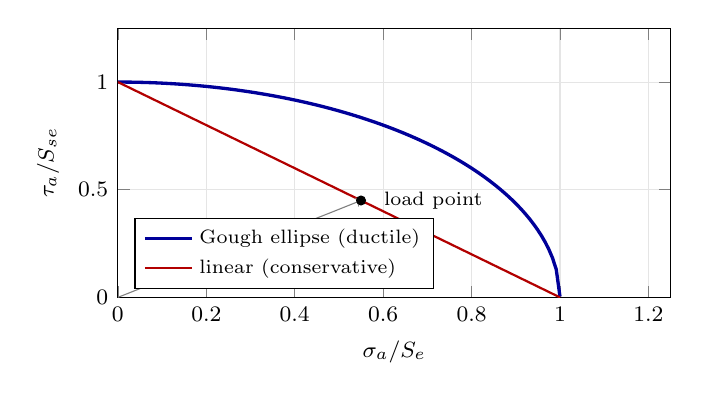
\begin{tikzpicture}
\begin{axis}[width=8.6cm,height=5.0cm,xlabel={$\sigma_a/S_e$},ylabel={$\tau_a/S_{se}$},
 xmin=0,xmax=1.25,ymin=0,ymax=1.25,grid=both,grid style={gray!20},
 label style={font=\footnotesize},tick label style={font=\footnotesize},
 legend pos=south west,legend style={font=\scriptsize},legend cell align=left]
\addplot[very thick,blue!60!black,domain=0:1,samples=120]{sqrt(1-x^2)};
\addlegendentry{Gough ellipse (ductile)}
\addplot[thick,red!70!black,domain=0:1,samples=2]{1-x};
\addlegendentry{linear (conservative)}
\addplot[only marks,mark=*,mark size=1.6pt,black] coordinates {(0.55,0.45)};
\node[font=\scriptsize,anchor=west] at (axis cs:0.58,0.45) {load point};
\draw[->,gray] (axis cs:0,0) -- (axis cs:0.55,0.45);
\end{axis}
\end{tikzpicture}